\documentclass[1p]{elsarticle_modified}
%\bibliographystyle{elsarticle-num}

%\usepackage[colorlinks]{hyperref}
%\usepackage{abbrmath_seonhwa} %\Abb, \Ascr, \Acal ,\Abf, \Afrak
\usepackage{amsfonts}
\usepackage{amssymb}
\usepackage{amsmath}
\usepackage{amsthm}
\usepackage{scalefnt}
\usepackage{amsbsy}
\usepackage{kotex}
\usepackage{caption}
\usepackage{subfig}
\usepackage{color}
\usepackage{graphicx}
\usepackage{xcolor} %% white, black, red, green, blue, cyan, magenta, yellow
\usepackage{float}
\usepackage{setspace}
\usepackage{hyperref}

\usepackage{tikz}
\usetikzlibrary{arrows}

\usepackage{multirow}
\usepackage{array} % fixed length table
\usepackage{hhline}

%%%%%%%%%%%%%%%%%%%%%
\makeatletter
\renewcommand*\env@matrix[1][\arraystretch]{%
	\edef\arraystretch{#1}%
	\hskip -\arraycolsep
	\let\@ifnextchar\new@ifnextchar
	\array{*\c@MaxMatrixCols c}}
\makeatother %https://tex.stackexchange.com/questions/14071/how-can-i-increase-the-line-spacing-in-a-matrix
%%%%%%%%%%%%%%%

\usepackage[normalem]{ulem}

\newcommand{\msout}[1]{\ifmmode\text{\sout{\ensuremath{#1}}}\else\sout{#1}\fi}
%SOURCE: \msout is \stkout macro in https://tex.stackexchange.com/questions/20609/strikeout-in-math-mode

\newcommand{\cancel}[1]{
	\ifmmode
	{\color{red}\msout{#1}}
	\else
	{\color{red}\sout{#1}}
	\fi
}

\newcommand{\add}[1]{
	{\color{blue}\uwave{#1}}
}

\newcommand{\replace}[2]{
	\ifmmode
	{\color{red}\msout{#1}}{\color{blue}\uwave{#2}}
	\else
	{\color{red}\sout{#1}}{\color{blue}\uwave{#2}}
	\fi
}

\newcommand{\Sol}{\mathcal{S}} %segment
\newcommand{\D}{D} %diagram
\newcommand{\A}{\mathcal{A}} %arc


%%%%%%%%%%%%%%%%%%%%%%%%%%%%%5 test

\def\sl{\operatorname{\textup{SL}}(2,\Cbb)}
\def\psl{\operatorname{\textup{PSL}}(2,\Cbb)}
\def\quan{\mkern 1mu \triangleright \mkern 1mu}

\theoremstyle{definition}
\newtheorem{thm}{Theorem}[section]
\newtheorem{prop}[thm]{Proposition}
\newtheorem{lem}[thm]{Lemma}
\newtheorem{ques}[thm]{Question}
\newtheorem{cor}[thm]{Corollary}
\newtheorem{defn}[thm]{Definition}
\newtheorem{exam}[thm]{Example}
\newtheorem{rmk}[thm]{Remark}
\newtheorem{alg}[thm]{Algorithm}

\newcommand{\I}{\sqrt{-1}}
\begin{document}

%\begin{frontmatter}
%
%\title{Boundary parabolic representations of knots up to 8 crossings}
%
%%% Group authors per affiliation:
%\author{Yunhi Cho} 
%\address{Department of Mathematics, University of Seoul, Seoul, Korea}
%\ead{yhcho@uos.ac.kr}
%
%
%\author{Seonhwa Kim} %\fnref{s_kim}}
%\address{Center for Geometry and Physics, Institute for Basic Science, Pohang, 37673, Korea}
%\ead{ryeona17@ibs.re.kr}
%
%\author{Hyuk Kim}
%\address{Department of Mathematical Sciences, Seoul National University, Seoul 08826, Korea}
%\ead{hyukkim@snu.ac.kr}
%
%\author{Seokbeom Yoon}
%\address{Department of Mathematical Sciences, Seoul National University, Seoul, 08826,  Korea}
%\ead{sbyoon15@snu.ac.kr}
%
%\begin{abstract}
%We find all boundary parabolic representation of knots up to 8 crossings.
%
%\end{abstract}
%\begin{keyword}
%    \MSC[2010] 57M25 
%\end{keyword}
%
%\end{frontmatter}

%\linenumbers
%\tableofcontents
%
\newcommand\colored[1]{\textcolor{white}{\rule[-0.35ex]{0.8em}{1.4ex}}\kern-0.8em\color{red} #1}%
%\newcommand\colored[1]{\textcolor{white}{ #1}\kern-2.17ex	\textcolor{white}{ #1}\kern-1.81ex	\textcolor{white}{ #1}\kern-2.15ex\color{red}#1	}

{\Large $\underline{12a_{0206}~(K12a_{0206})}$}

\setlength{\tabcolsep}{10pt}
\renewcommand{\arraystretch}{1.6}
\vspace{1cm}\begin{tabular}{m{100pt}>{\centering\arraybackslash}m{274pt}}
\multirow{5}{120pt}{
	\centering
	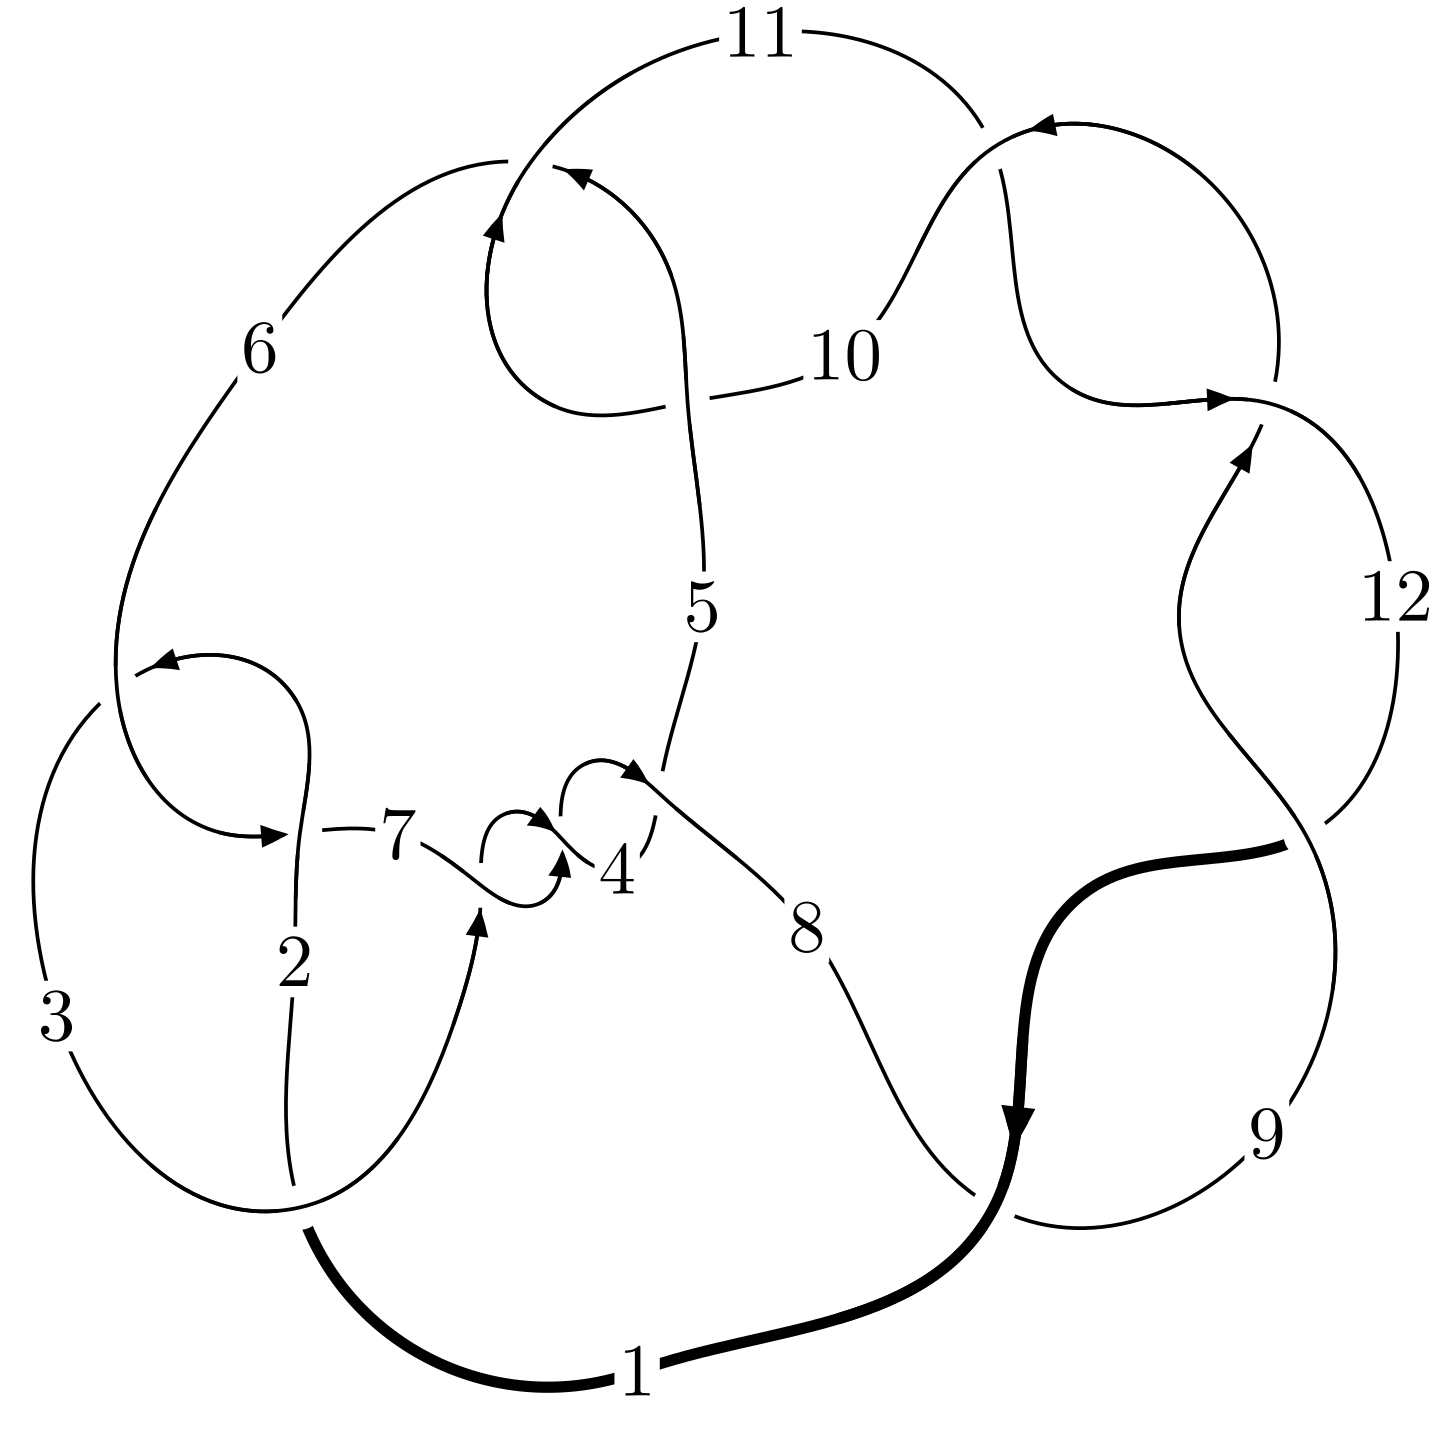
\includegraphics[width=112pt]{../../../GIT/diagram.site/Diagrams/png/1007_12a_0206.png}\\
\ \ \ A knot diagram\footnotemark}&
\allowdisplaybreaks
\textbf{Linearized knot diagam} \\
\cline{2-2}
 &
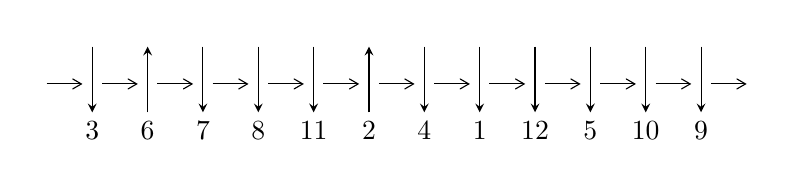
\begin{tikzpicture}[x=20pt, y=17pt]
	% nodes
	\node (C0) at (0, 0) {};
	\node (C1) at (1, 0) {};
	\node (C1U) at (1, +1) {};
	\node (C1D) at (1, -1) {3};

	\node (C2) at (2, 0) {};
	\node (C2U) at (2, +1) {};
	\node (C2D) at (2, -1) {6};

	\node (C3) at (3, 0) {};
	\node (C3U) at (3, +1) {};
	\node (C3D) at (3, -1) {7};

	\node (C4) at (4, 0) {};
	\node (C4U) at (4, +1) {};
	\node (C4D) at (4, -1) {8};

	\node (C5) at (5, 0) {};
	\node (C5U) at (5, +1) {};
	\node (C5D) at (5, -1) {11};

	\node (C6) at (6, 0) {};
	\node (C6U) at (6, +1) {};
	\node (C6D) at (6, -1) {2};

	\node (C7) at (7, 0) {};
	\node (C7U) at (7, +1) {};
	\node (C7D) at (7, -1) {4};

	\node (C8) at (8, 0) {};
	\node (C8U) at (8, +1) {};
	\node (C8D) at (8, -1) {1};

	\node (C9) at (9, 0) {};
	\node (C9U) at (9, +1) {};
	\node (C9D) at (9, -1) {12};

	\node (C10) at (10, 0) {};
	\node (C10U) at (10, +1) {};
	\node (C10D) at (10, -1) {5};

	\node (C11) at (11, 0) {};
	\node (C11U) at (11, +1) {};
	\node (C11D) at (11, -1) {10};

	\node (C12) at (12, 0) {};
	\node (C12U) at (12, +1) {};
	\node (C12D) at (12, -1) {9};
	\node (C13) at (13, 0) {};

	% arrows
	\draw[->,>={angle 60}]
	(C0) edge (C1) (C1) edge (C2) (C2) edge (C3) (C3) edge (C4) (C4) edge (C5) (C5) edge (C6) (C6) edge (C7) (C7) edge (C8) (C8) edge (C9) (C9) edge (C10) (C10) edge (C11) (C11) edge (C12) (C12) edge (C13) ;	\draw[->,>=stealth]
	(C1U) edge (C1D) (C2D) edge (C2U) (C3U) edge (C3D) (C4U) edge (C4D) (C5U) edge (C5D) (C6D) edge (C6U) (C7U) edge (C7D) (C8U) edge (C8D) (C9U) edge (C9D) (C10U) edge (C10D) (C11U) edge (C11D) (C12U) edge (C12D) ;
	\end{tikzpicture} \\
\hhline{~~} \\& 
\textbf{Solving Sequence} \\ \cline{2-2} 
 &
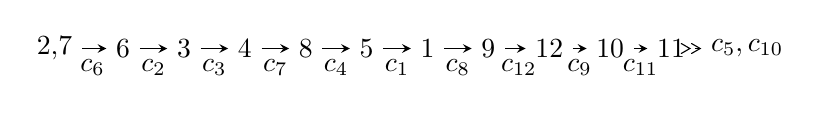
\begin{tikzpicture}[x=22pt, y=7pt]
	% node
	\node (A0) at (-1/8, 0) {2,7};
	\node (A1) at (1, 0) {6};
	\node (A2) at (2, 0) {3};
	\node (A3) at (3, 0) {4};
	\node (A4) at (4, 0) {8};
	\node (A5) at (5, 0) {5};
	\node (A6) at (6, 0) {1};
	\node (A7) at (7, 0) {9};
	\node (A8) at (8, 0) {12};
	\node (A9) at (9, 0) {10};
	\node (A10) at (10, 0) {11};
	\node (C1) at (1/2, -1) {$c_{6}$};
	\node (C2) at (3/2, -1) {$c_{2}$};
	\node (C3) at (5/2, -1) {$c_{3}$};
	\node (C4) at (7/2, -1) {$c_{7}$};
	\node (C5) at (9/2, -1) {$c_{4}$};
	\node (C6) at (11/2, -1) {$c_{1}$};
	\node (C7) at (13/2, -1) {$c_{8}$};
	\node (C8) at (15/2, -1) {$c_{12}$};
	\node (C9) at (17/2, -1) {$c_{9}$};
	\node (C10) at (19/2, -1) {$c_{11}$};
	\node (A11) at (45/4, 0) {$c_{5},c_{10}$};

	% edge
	\draw[->,>=stealth]	
	(A0) edge (A1) (A1) edge (A2) (A2) edge (A3) (A3) edge (A4) (A4) edge (A5) (A5) edge (A6) (A6) edge (A7) (A7) edge (A8) (A8) edge (A9) (A9) edge (A10) ;
	\draw[->>,>={angle 60}]	
	(A10) edge (A11);
\end{tikzpicture} \\ 

\end{tabular} \\

\footnotetext{
The image of knot diagram is generated by the software ``\textbf{Draw programme}" developed by Andrew Bartholomew(\url{http://www.layer8.co.uk/maths/draw/index.htm\#Running-draw}), where we modified some parts for our purpose(\url{https://github.com/CATsTAILs/LinksPainter}).
}\phantom \\ \newline 
\centering \textbf{Ideals for irreducible components\footnotemark of $X_{\text{par}}$} 
 
\begin{align*}
I^u_{1}&=\langle 
u^{52}+u^{51}+\cdots+2 u-1\rangle \\
\\
\end{align*}
\raggedright * 1 irreducible components of $\dim_{\mathbb{C}}=0$, with total 52 representations.\\
\footnotetext{All coefficients of polynomials are rational numbers. But the coefficients are sometimes approximated in decimal forms when there is not enough margin.}
\newpage
\renewcommand{\arraystretch}{1}
\centering \section*{I. $I^u_{1}= \langle u^{52}+u^{51}+\cdots+2 u-1 \rangle$}
\flushleft \textbf{(i) Arc colorings}\\
\begin{tabular}{m{7pt} m{180pt} m{7pt} m{180pt} }
\flushright $a_{2}=$&$\begin{pmatrix}0\\u\end{pmatrix}$ \\
\flushright $a_{7}=$&$\begin{pmatrix}1\\0\end{pmatrix}$ \\
\flushright $a_{6}=$&$\begin{pmatrix}1\\u^2\end{pmatrix}$ \\
\flushright $a_{3}=$&$\begin{pmatrix}u\\u^3+u\end{pmatrix}$ \\
\flushright $a_{4}=$&$\begin{pmatrix}- u^3\\u^3+u\end{pmatrix}$ \\
\flushright $a_{8}=$&$\begin{pmatrix}- u^6- u^4+1\\u^6+2 u^4+u^2\end{pmatrix}$ \\
\flushright $a_{5}=$&$\begin{pmatrix}u^9+2 u^7+u^5-2 u^3- u\\- u^9-3 u^7-3 u^5+u\end{pmatrix}$ \\
\flushright $a_{1}=$&$\begin{pmatrix}u^3\\u^5+u^3+u\end{pmatrix}$ \\
\flushright $a_{9}=$&$\begin{pmatrix}- u^{14}-3 u^{12}-4 u^{10}- u^8+1\\- u^{16}-4 u^{14}-8 u^{12}-8 u^{10}-4 u^8+2 u^6+4 u^4+2 u^2\end{pmatrix}$ \\
\flushright $a_{12}=$&$\begin{pmatrix}u^{25}+6 u^{23}+\cdots+2 u^3+u\\u^{27}+7 u^{25}+\cdots+3 u^3+u\end{pmatrix}$ \\
\flushright $a_{10}=$&$\begin{pmatrix}- u^{36}-9 u^{34}+\cdots+u^2+1\\- u^{38}-10 u^{36}+\cdots+8 u^4+3 u^2\end{pmatrix}$ \\
\flushright $a_{11}=$&$\begin{pmatrix}u^{47}+12 u^{45}+\cdots+4 u^3+2 u\\u^{49}+13 u^{47}+\cdots+6 u^3+u\end{pmatrix}$\\&\end{tabular}
\flushleft \textbf{(ii) Obstruction class $= -1$}\\~\\
\flushleft \textbf{(iii) Cusp Shapes $= -4 u^{51}-4 u^{50}+\cdots+16 u-14$}\\~\\
\newpage\renewcommand{\arraystretch}{1}
\flushleft \textbf{(iv) u-Polynomials at the component}\newline \\
\begin{tabular}{m{50pt}|m{274pt}}
Crossings & \hspace{64pt}u-Polynomials at each crossing \\
\hline $$\begin{aligned}c_{1}\end{aligned}$$&$\begin{aligned}
&u^{52}+29 u^{51}+\cdots-2 u+1
\end{aligned}$\\
\hline $$\begin{aligned}c_{2},c_{6}\end{aligned}$$&$\begin{aligned}
&u^{52}- u^{51}+\cdots-2 u-1
\end{aligned}$\\
\hline $$\begin{aligned}c_{3},c_{4},c_{7}\end{aligned}$$&$\begin{aligned}
&u^{52}+u^{51}+\cdots+9 u-2
\end{aligned}$\\
\hline $$\begin{aligned}c_{5},c_{10}\end{aligned}$$&$\begin{aligned}
&u^{52}+u^{51}+\cdots-2 u-1
\end{aligned}$\\
\hline $$\begin{aligned}c_{8},c_{9},c_{11}\\c_{12}\end{aligned}$$&$\begin{aligned}
&u^{52}+11 u^{51}+\cdots+2 u+1
\end{aligned}$\\
\hline
\end{tabular}\\~\\
\newpage\renewcommand{\arraystretch}{1}
\flushleft \textbf{(v) Riley Polynomials at the component}\newline \\
\begin{tabular}{m{50pt}|m{274pt}}
Crossings & \hspace{64pt}Riley Polynomials at each crossing \\
\hline $$\begin{aligned}c_{1}\end{aligned}$$&$\begin{aligned}
&y^{52}-11 y^{51}+\cdots-54 y+1
\end{aligned}$\\
\hline $$\begin{aligned}c_{2},c_{6}\end{aligned}$$&$\begin{aligned}
&y^{52}+29 y^{51}+\cdots-2 y+1
\end{aligned}$\\
\hline $$\begin{aligned}c_{3},c_{4},c_{7}\end{aligned}$$&$\begin{aligned}
&y^{52}-51 y^{51}+\cdots+115 y+4
\end{aligned}$\\
\hline $$\begin{aligned}c_{5},c_{10}\end{aligned}$$&$\begin{aligned}
&y^{52}-11 y^{51}+\cdots-2 y+1
\end{aligned}$\\
\hline $$\begin{aligned}c_{8},c_{9},c_{11}\\c_{12}\end{aligned}$$&$\begin{aligned}
&y^{52}+61 y^{51}+\cdots+2 y+1
\end{aligned}$\\
\hline
\end{tabular}\\~\\
\newpage\flushleft \textbf{(vi) Complex Volumes and Cusp Shapes}
$$\begin{array}{c|c|c}  
\text{Solutions to }I^u_{1}& \I (\text{vol} + \sqrt{-1}CS) & \text{Cusp shape}\\
 \hline 
\begin{aligned}
u &= -0.444793 + 0.901226 I\end{aligned}
 & \phantom{-}0.92885 - 2.07964 I & -4.26783 + 3.51699 I \\ \hline\begin{aligned}
u &= -0.444793 - 0.901226 I\end{aligned}
 & \phantom{-}0.92885 + 2.07964 I & -4.26783 - 3.51699 I \\ \hline\begin{aligned}
u &= \phantom{-}0.146457 + 0.972329 I\end{aligned}
 & -1.98877 - 1.22586 I & -14.2459 + 3.8733 I \\ \hline\begin{aligned}
u &= \phantom{-}0.146457 - 0.972329 I\end{aligned}
 & -1.98877 + 1.22586 I & -14.2459 - 3.8733 I \\ \hline\begin{aligned}
u &= \phantom{-}0.323497 + 0.988659 I\end{aligned}
 & -3.15249 + 2.68021 I & -16.7312 - 6.1438 I \\ \hline\begin{aligned}
u &= \phantom{-}0.323497 - 0.988659 I\end{aligned}
 & -3.15249 - 2.68021 I & -16.7312 + 6.1438 I \\ \hline\begin{aligned}
u &= \phantom{-}0.456989 + 0.963997 I\end{aligned}
 & \phantom{-}0.08024 + 6.29340 I & -7.80687 - 10.48412 I \\ \hline\begin{aligned}
u &= \phantom{-}0.456989 - 0.963997 I\end{aligned}
 & \phantom{-}0.08024 - 6.29340 I & -7.80687 + 10.48412 I \\ \hline\begin{aligned}
u &= -0.533289 + 0.935620 I\end{aligned}
 & \phantom{-}8.97543 - 1.96457 I & -4.12437 + 3.29680 I \\ \hline\begin{aligned}
u &= -0.533289 - 0.935620 I\end{aligned}
 & \phantom{-}8.97543 + 1.96457 I & -4.12437 - 3.29680 I \\ \hline\begin{aligned}
u &= \phantom{-}0.010867 + 1.083970 I\end{aligned}
 & \phantom{-}5.22663 - 3.18836 I & -9.99011 + 2.49513 I \\ \hline\begin{aligned}
u &= \phantom{-}0.010867 - 1.083970 I\end{aligned}
 & \phantom{-}5.22663 + 3.18836 I & -9.99011 - 2.49513 I \\ \hline\begin{aligned}
u &= \phantom{-}0.533053 + 0.946195 I\end{aligned}
 & \phantom{-}8.84021 + 8.51151 I & -4.50581 - 8.08698 I \\ \hline\begin{aligned}
u &= \phantom{-}0.533053 - 0.946195 I\end{aligned}
 & \phantom{-}8.84021 - 8.51151 I & -4.50581 + 8.08698 I \\ \hline\begin{aligned}
u &= -0.286778 + 0.838173 I\end{aligned}
 & -0.49981 - 1.35692 I & -5.02302 + 4.66234 I \\ \hline\begin{aligned}
u &= -0.286778 - 0.838173 I\end{aligned}
 & -0.49981 + 1.35692 I & -5.02302 - 4.66234 I \\ \hline\begin{aligned}
u &= -0.844411 + 0.100508 I\end{aligned}
 & \phantom{-}4.53747 + 8.38588 I & -5.64729 - 5.07323 I \\ \hline\begin{aligned}
u &= -0.844411 - 0.100508 I\end{aligned}
 & \phantom{-}4.53747 - 8.38588 I & -5.64729 + 5.07323 I \\ \hline\begin{aligned}
u &= \phantom{-}0.835966 + 0.104158 I\end{aligned}
 & \phantom{-}4.83277 - 1.89906 I & -5.09326 + 0.33485 I \\ \hline\begin{aligned}
u &= \phantom{-}0.835966 - 0.104158 I\end{aligned}
 & \phantom{-}4.83277 + 1.89906 I & -5.09326 - 0.33485 I \\ \hline\begin{aligned}
u &= -0.836110 + 0.052296 I\end{aligned}
 & -3.96880 + 5.07450 I & -9.58177 - 6.04455 I \\ \hline\begin{aligned}
u &= -0.836110 - 0.052296 I\end{aligned}
 & -3.96880 - 5.07450 I & -9.58177 + 6.04455 I \\ \hline\begin{aligned}
u &= -0.837189\phantom{ +0.000000I}\end{aligned}
 & -6.56025\phantom{ +0.000000I} & -14.2030\phantom{ +0.000000I} \\ \hline\begin{aligned}
u &= \phantom{-}0.800491 + 0.040631 I\end{aligned}
 & -2.27501 - 0.99664 I & -5.31105 + 0.16572 I \\ \hline\begin{aligned}
u &= \phantom{-}0.800491 - 0.040631 I\end{aligned}
 & -2.27501 + 0.99664 I & -5.31105 - 0.16572 I \\ \hline\begin{aligned}
u &= -0.590815 + 0.525994 I\end{aligned}
 & \phantom{-}10.12740 - 2.48798 I & -1.62823 + 2.66940 I \\ \hline\begin{aligned}
u &= -0.590815 - 0.525994 I\end{aligned}
 & \phantom{-}10.12740 + 2.48798 I & -1.62823 - 2.66940 I \\ \hline\begin{aligned}
u &= \phantom{-}0.595814 + 0.510152 I\end{aligned}
 & \phantom{-}10.06680 - 4.04960 I & -1.78451 + 2.29010 I \\ \hline\begin{aligned}
u &= \phantom{-}0.595814 - 0.510152 I\end{aligned}
 & \phantom{-}10.06680 + 4.04960 I & -1.78451 - 2.29010 I \\ \hline\begin{aligned}
u &= \phantom{-}0.440029 + 1.215220 I\end{aligned}
 & -5.96613 + 3.38286 I & \phantom{-0.000000 } 0\\
 \hline 
 \end{array}$$\newpage$$\begin{array}{c|c|c}  
\text{Solutions to }I^u_{1}& \I (\text{vol} + \sqrt{-1}CS) & \text{Cusp shape}\\
 \hline 
\begin{aligned}
u &= \phantom{-}0.440029 - 1.215220 I\end{aligned}
 & -5.96613 - 3.38286 I & \phantom{-0.000000 } 0 \\ \hline\begin{aligned}
u &= -0.436602 + 0.554857 I\end{aligned}
 & \phantom{-}1.87781 - 1.71309 I & -1.63672 + 4.44020 I \\ \hline\begin{aligned}
u &= -0.436602 - 0.554857 I\end{aligned}
 & \phantom{-}1.87781 + 1.71309 I & -1.63672 - 4.44020 I \\ \hline\begin{aligned}
u &= \phantom{-}0.399851 + 1.232500 I\end{aligned}
 & \phantom{-}0.78270 + 2.35026 I & \phantom{-0.000000 } 0 \\ \hline\begin{aligned}
u &= \phantom{-}0.399851 - 1.232500 I\end{aligned}
 & \phantom{-}0.78270 - 2.35026 I & \phantom{-0.000000 } 0 \\ \hline\begin{aligned}
u &= \phantom{-}0.474496 + 1.211950 I\end{aligned}
 & -5.71832 + 5.61366 I & \phantom{-0.000000 } 0 \\ \hline\begin{aligned}
u &= \phantom{-}0.474496 - 1.211950 I\end{aligned}
 & -5.71832 - 5.61366 I & \phantom{-0.000000 } 0 \\ \hline\begin{aligned}
u &= -0.402451 + 1.238770 I\end{aligned}
 & \phantom{-}0.46667 + 4.08632 I & \phantom{-0.000000 } 0 \\ \hline\begin{aligned}
u &= -0.402451 - 1.238770 I\end{aligned}
 & \phantom{-}0.46667 - 4.08632 I & \phantom{-0.000000 } 0 \\ \hline\begin{aligned}
u &= -0.432707 + 1.233580 I\end{aligned}
 & -7.82605 + 0.62175 I & \phantom{-0.000000 } 0 \\ \hline\begin{aligned}
u &= -0.432707 - 1.233580 I\end{aligned}
 & -7.82605 - 0.62175 I & \phantom{-0.000000 } 0 \\ \hline\begin{aligned}
u &= -0.459952 + 1.231280 I\end{aligned}
 & -10.23690 - 4.62494 I & \phantom{-0.000000 } 0 \\ \hline\begin{aligned}
u &= -0.459952 - 1.231280 I\end{aligned}
 & -10.23690 + 4.62494 I & \phantom{-0.000000 } 0 \\ \hline\begin{aligned}
u &= \phantom{-}0.504700 + 1.214320 I\end{aligned}
 & \phantom{-}1.52858 + 6.77648 I & \phantom{-0.000000 } 0 \\ \hline\begin{aligned}
u &= \phantom{-}0.504700 - 1.214320 I\end{aligned}
 & \phantom{-}1.52858 - 6.77648 I & \phantom{-0.000000 } 0 \\ \hline\begin{aligned}
u &= -0.483738 + 1.224360 I\end{aligned}
 & -7.45916 - 9.83676 I & \phantom{-0.000000 } 0 \\ \hline\begin{aligned}
u &= -0.483738 - 1.224360 I\end{aligned}
 & -7.45916 + 9.83676 I & \phantom{-0.000000 } 0 \\ \hline\begin{aligned}
u &= -0.505337 + 1.218480 I\end{aligned}
 & \phantom{-}1.20269 - 13.28750 I & \phantom{-0.000000 } 0 \\ \hline\begin{aligned}
u &= -0.505337 - 1.218480 I\end{aligned}
 & \phantom{-}1.20269 + 13.28750 I & \phantom{-0.000000 } 0 \\ \hline\begin{aligned}
u &= \phantom{-}0.475410 + 0.418845 I\end{aligned}
 & \phantom{-}1.55220 - 2.39312 I & -3.19595 + 4.86079 I \\ \hline\begin{aligned}
u &= \phantom{-}0.475410 - 0.418845 I\end{aligned}
 & \phantom{-}1.55220 + 2.39312 I & -3.19595 - 4.86079 I \\ \hline\begin{aligned}
u &= \phantom{-}0.355912\phantom{ +0.000000I}\end{aligned}
 & -0.860619\phantom{ +0.000000I} & -11.7250\phantom{ +0.000000I}\\
 \hline 
 \end{array}$$\newpage
\newpage\renewcommand{\arraystretch}{1}
\centering \section*{ II. u-Polynomials}
\begin{tabular}{m{50pt}|m{274pt}}
Crossings & \hspace{64pt}u-Polynomials at each crossing \\
\hline $$\begin{aligned}c_{1}\end{aligned}$$&$\begin{aligned}
&u^{52}+29 u^{51}+\cdots-2 u+1
\end{aligned}$\\
\hline $$\begin{aligned}c_{2},c_{6}\end{aligned}$$&$\begin{aligned}
&u^{52}- u^{51}+\cdots-2 u-1
\end{aligned}$\\
\hline $$\begin{aligned}c_{3},c_{4},c_{7}\end{aligned}$$&$\begin{aligned}
&u^{52}+u^{51}+\cdots+9 u-2
\end{aligned}$\\
\hline $$\begin{aligned}c_{5},c_{10}\end{aligned}$$&$\begin{aligned}
&u^{52}+u^{51}+\cdots-2 u-1
\end{aligned}$\\
\hline $$\begin{aligned}c_{8},c_{9},c_{11}\\c_{12}\end{aligned}$$&$\begin{aligned}
&u^{52}+11 u^{51}+\cdots+2 u+1
\end{aligned}$\\
\hline
\end{tabular}\newpage\renewcommand{\arraystretch}{1}
\centering \section*{ III. Riley Polynomials}
\begin{tabular}{m{50pt}|m{274pt}}
Crossings & \hspace{64pt}Riley Polynomials at each crossing \\
\hline $$\begin{aligned}c_{1}\end{aligned}$$&$\begin{aligned}
&y^{52}-11 y^{51}+\cdots-54 y+1
\end{aligned}$\\
\hline $$\begin{aligned}c_{2},c_{6}\end{aligned}$$&$\begin{aligned}
&y^{52}+29 y^{51}+\cdots-2 y+1
\end{aligned}$\\
\hline $$\begin{aligned}c_{3},c_{4},c_{7}\end{aligned}$$&$\begin{aligned}
&y^{52}-51 y^{51}+\cdots+115 y+4
\end{aligned}$\\
\hline $$\begin{aligned}c_{5},c_{10}\end{aligned}$$&$\begin{aligned}
&y^{52}-11 y^{51}+\cdots-2 y+1
\end{aligned}$\\
\hline $$\begin{aligned}c_{8},c_{9},c_{11}\\c_{12}\end{aligned}$$&$\begin{aligned}
&y^{52}+61 y^{51}+\cdots+2 y+1
\end{aligned}$\\
\hline
\end{tabular}
\vskip 2pc
\end{document}